\chapter{Experimental Results}
\markright{experiments}
\label{exp}
\phantomsection
%\addcontentsline{toc}{chapter}{experiments}

The proposed method has been tested to verify, besides the uniqueness of the watermark, its validity in terms of robustness and perceptual impact.\newline As said before, robustness is the ability of the watermark to cope with the degradation of the image due to compression, view synthesis etc.\newline 
Another important feature of a good watermarking method is perceptual transparency, such that human eye could not distinguish the dissimilarities between the watermarked image and the original one.\newline In this chapter will be presented the results carried out to test the algorithm performances.\newline


The marking process has been applied to a 1 minute stereo-video sequence created starting from the left and right view of the New Tsukuba dataset \cite{tsu}, with GOP of 60 frames and 30 fps.\newline 
Its been chosen to mark every 60 frames, i.e. only the I frame of each GOP.\newline 
The frames of the reference video has been marked with different power and new marked videos has been created with different levels of compression.\newline 

The compressed videos are made with the \texttt{ffmpeg} library \cite{ffmapeg}, changing the Constant Rate Factor (CRF), the default quality setting for the x264 encoder. The value can be set in a range between 0 and 51, where lower values would result in better quality (at the expense of higher file sizes). 

\section{Uniqueness of the watermark}

The first experiment we present aims to demonstrate the uniqueness of the watermark: figures \ref{fig:Ll03}-\ref{fig:Lrnm} show the response of the watermark detector to 100 randomly generated watermarks of which only one matches the reference watermark. \newline The potive response due to the correct watermark is very much stronger with respect to the response to incorrect watermarks, suggesting that the algotithm has very low false positive (and false negative) response rate.
\begin{figure}[h!]
\centering
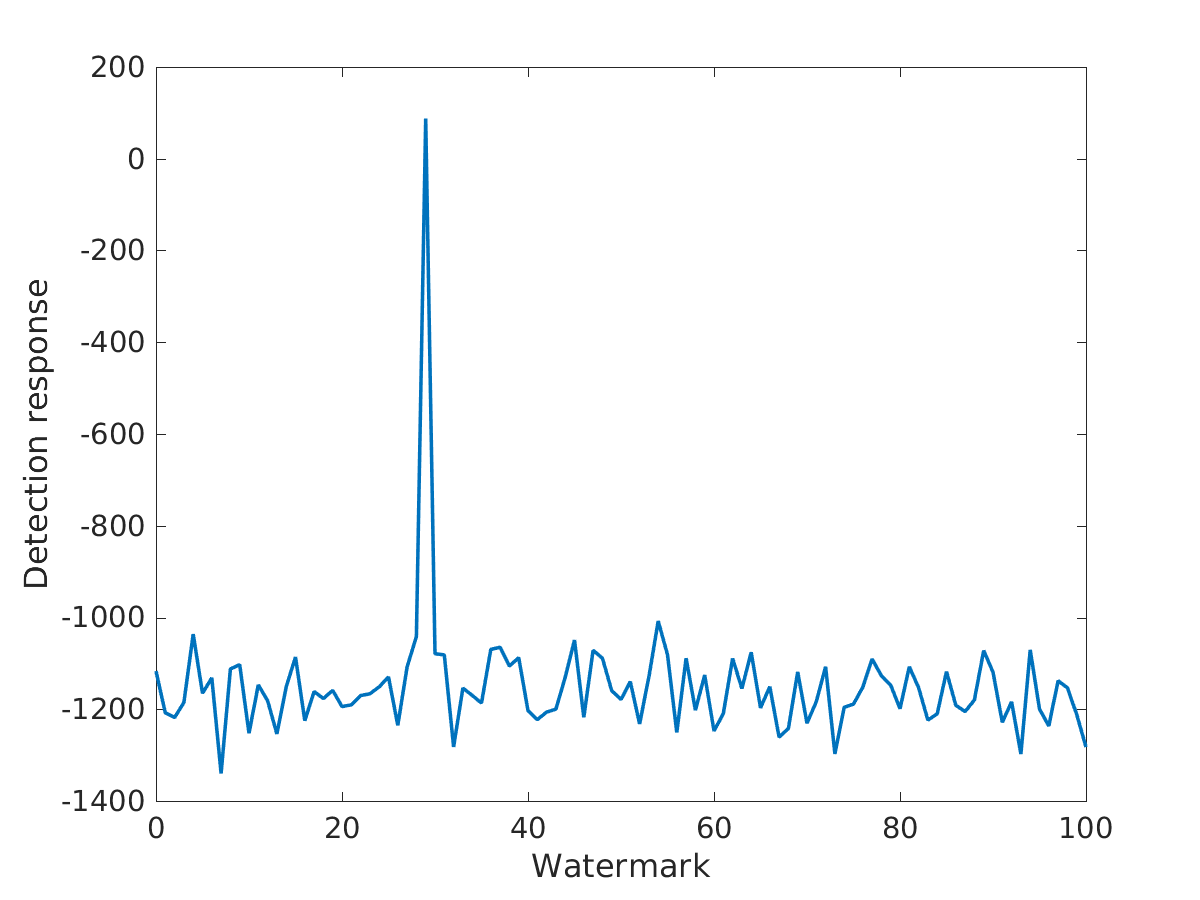
\includegraphics[width=0.4\textwidth]{./img/likelihood/correct_LikelihoodL_03.png}
\caption{\small{detector response on the left view marked with power equal to 0.3}}
\label{fig:Ll03}
\end{figure}
\begin{figure}[h!]
\centering
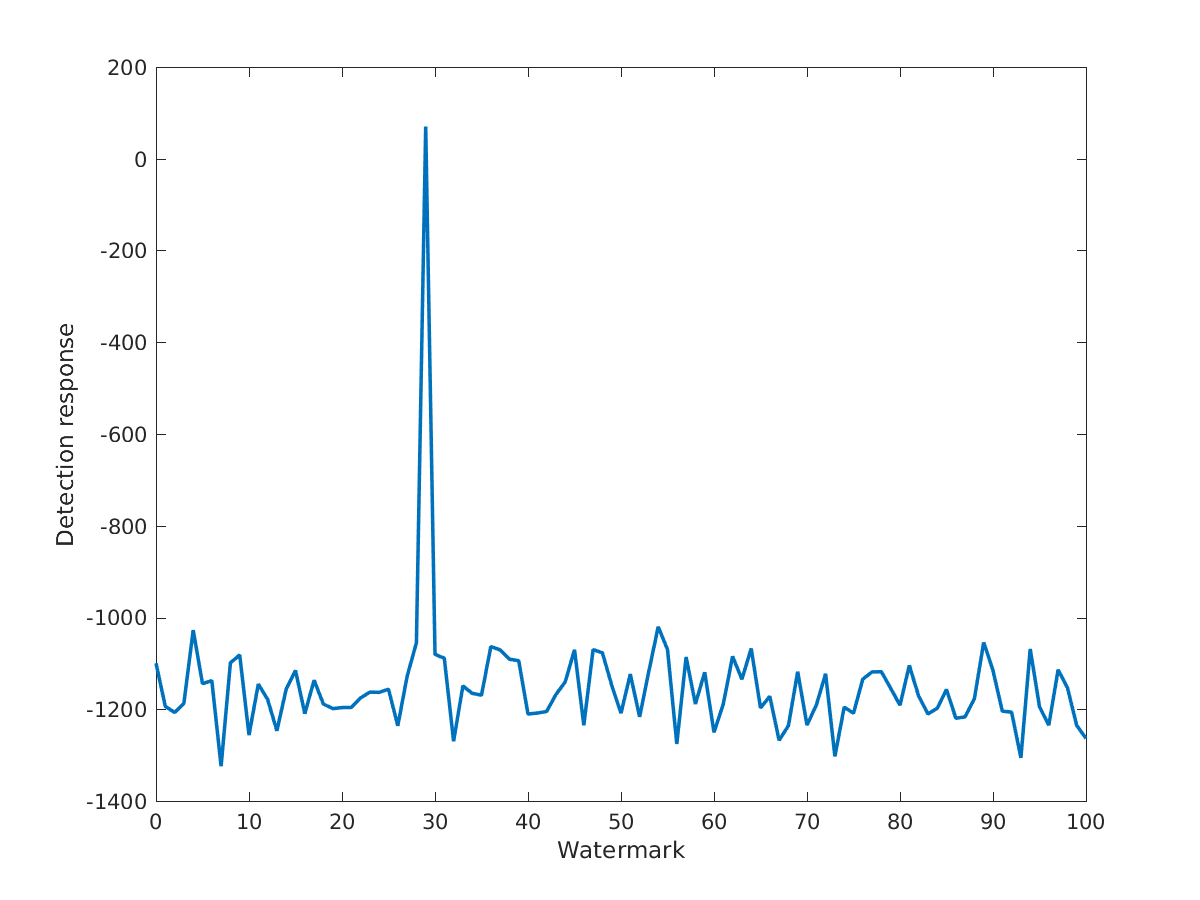
\includegraphics[width=0.4\textwidth]{./img/likelihood/correct_LikelihoodLr_03.png}
\caption{\small{detector response on the left view reconstructed from the right marked with power equal to 0.3}}
\label{fig:Lr03}
\end{figure}
\begin{figure}[h!]
\centering
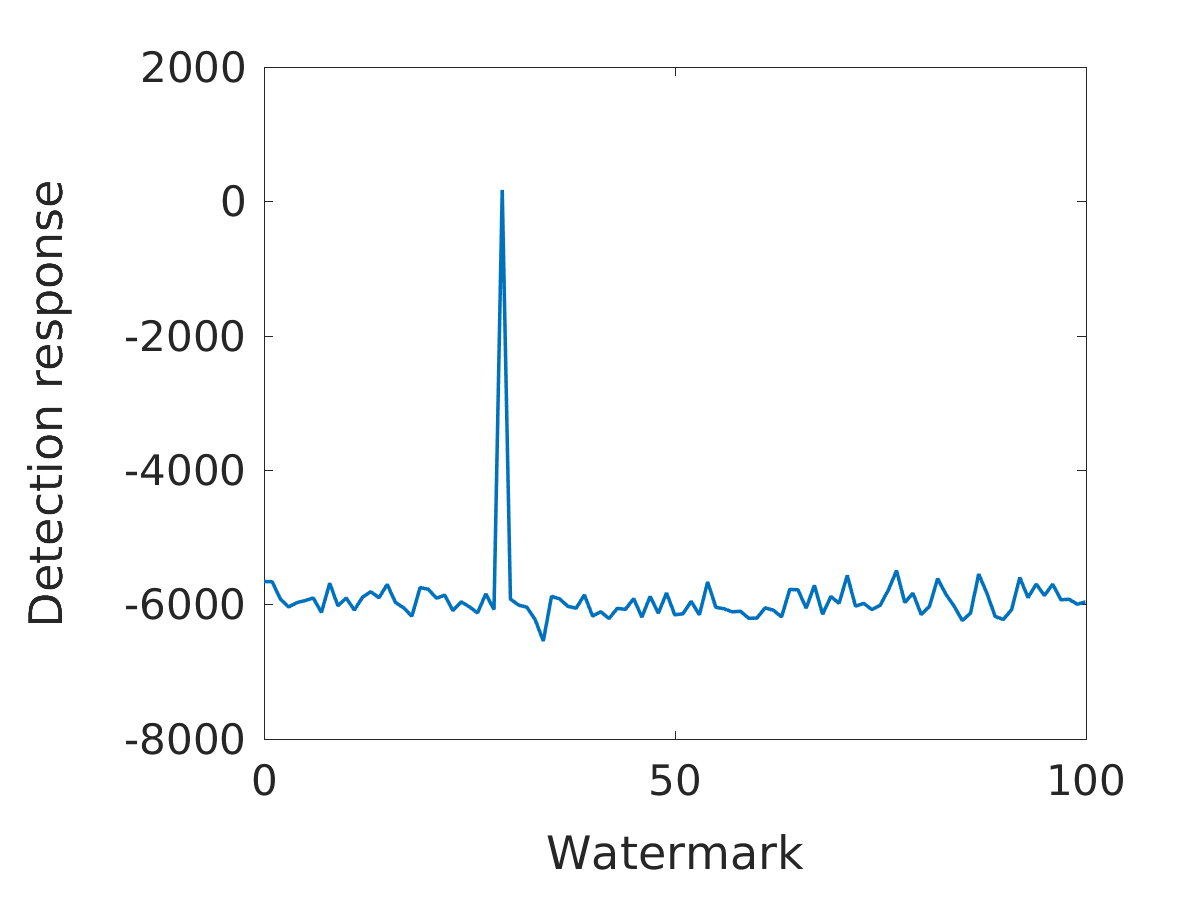
\includegraphics[width=0.4\textwidth]{./img/likelihood/correct_LikelihoodL_06.png}
\caption{\small{detector response on the left view marked with power equal to 0.6}}
\label{fig:Ll06}
\end{figure}
\begin{figure}[h!]
\centering
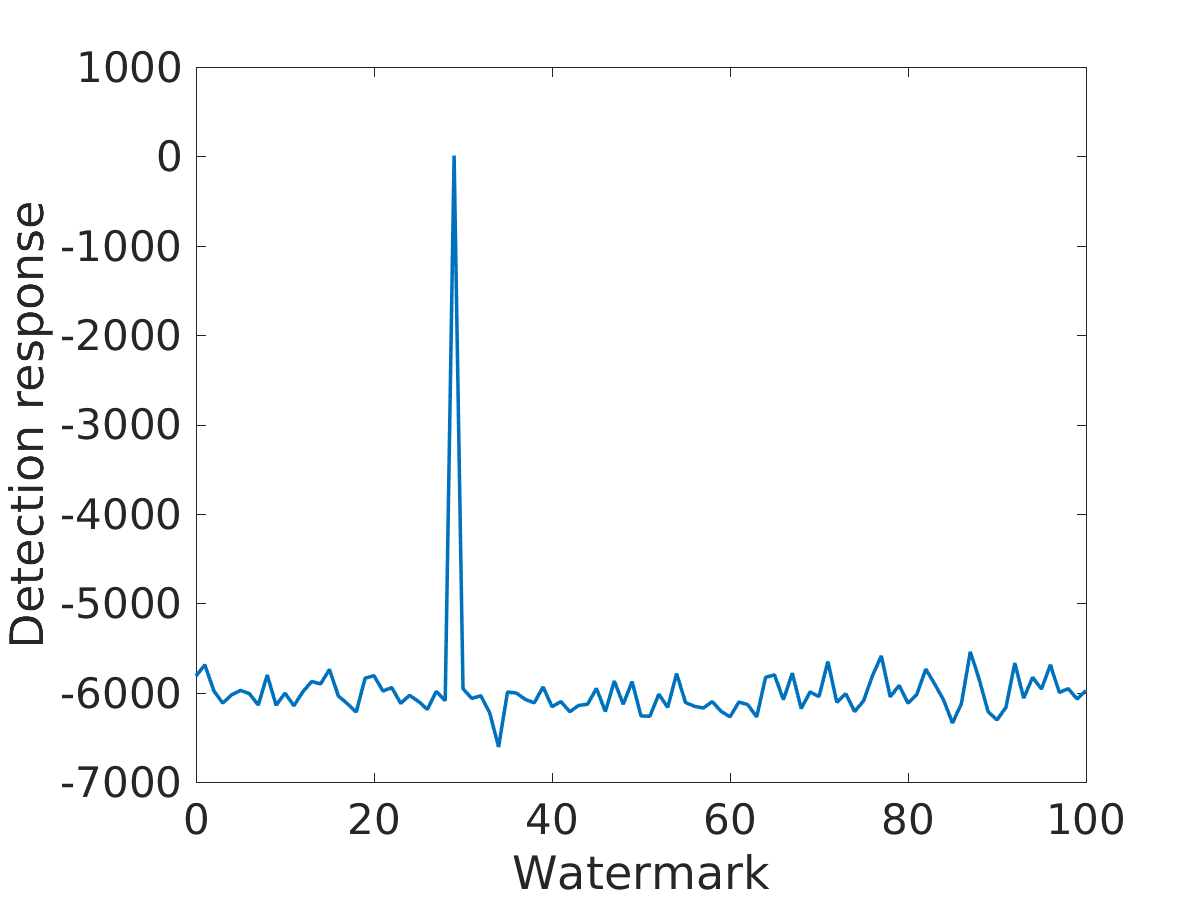
\includegraphics[width=0.4\textwidth]{./img/likelihood/correct_LikelihoodLr_06.png}
\caption{\small{detector response on the left view reconstructed from the right marked with power equal to 0.6}}
\label{fig:Lr06}
\end{figure}
\begin{figure}[h!]
\centering
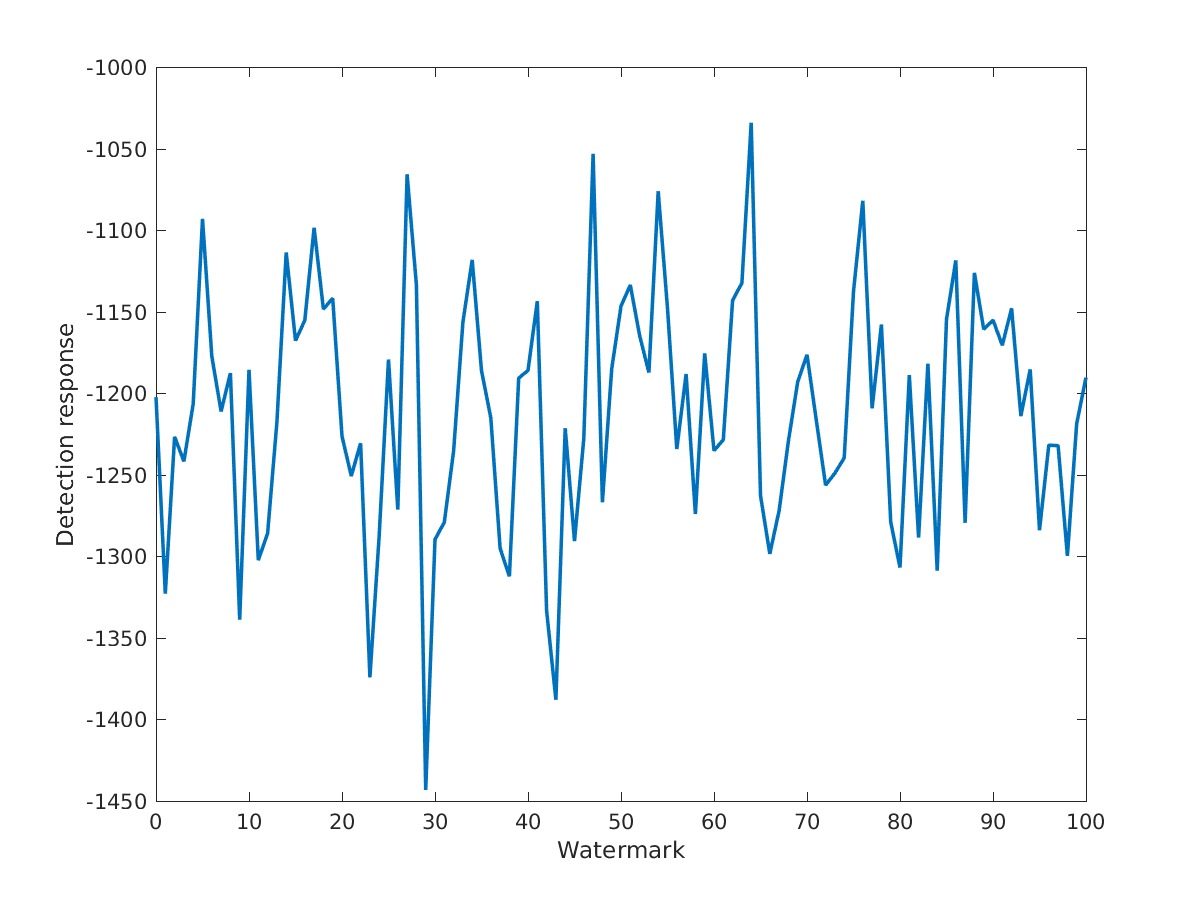
\includegraphics[width=0.4\textwidth]{./img/likelihood/correct_LikelihoodL_NM.png}
\caption{\small{detector response on the left view where the image hasn't been marked}}
\label{fig:Llnm}
\end{figure}
\begin{figure}[h!]
\centering
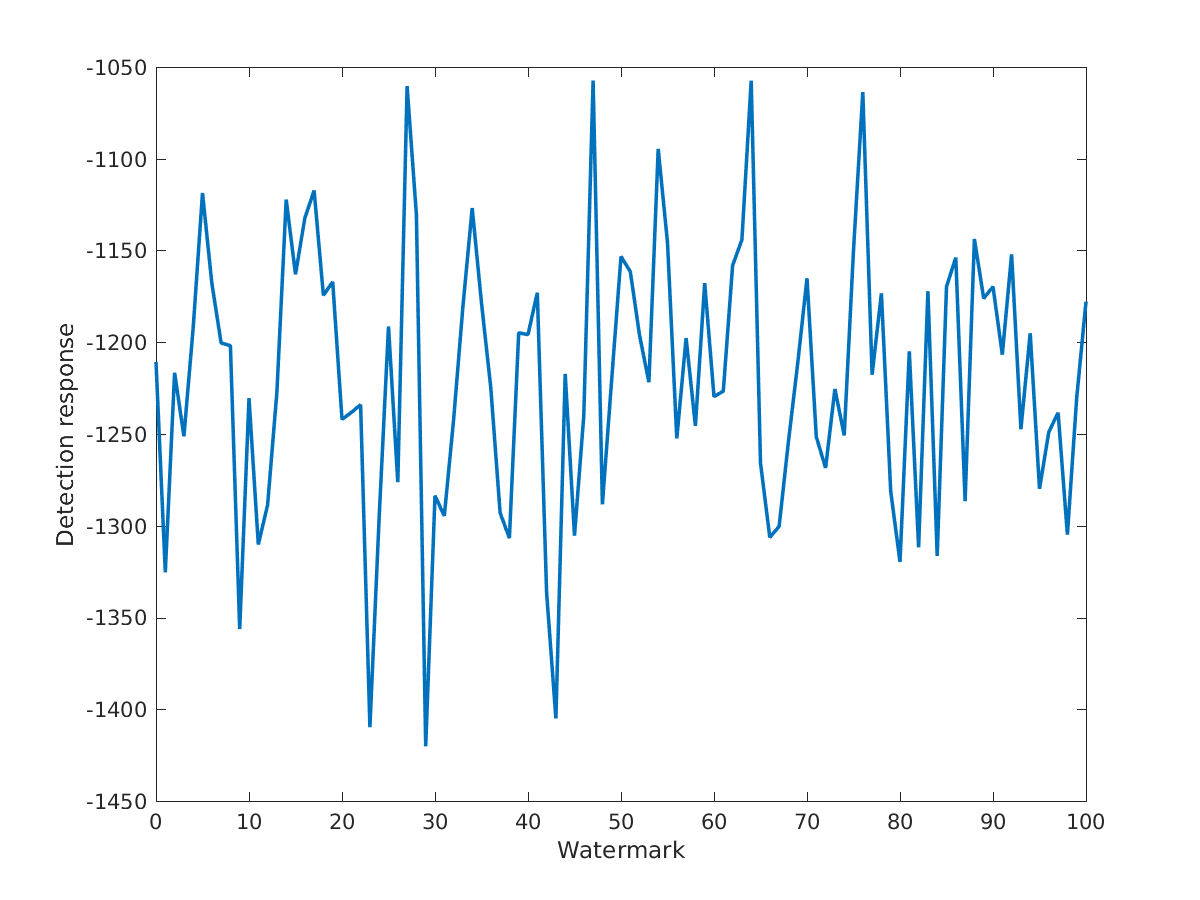
\includegraphics[width=0.4\textwidth]{./img/likelihood/correct_LikelihoodLr_NM.png}
\caption{\small{detector response on the left view reconstructed from the right where the image hasn't been marked}}
\label{fig:Lrnm}
\end{figure}
\clearpage


\section{Robustness against compression}

In video analysis, compression is useful because it helps reduce resource usage, such as data storage space or transmission capacity.\newline  This process brings to a degradation of the image due to the compression ratio, thus a degradation of the watermark.\newline  To prevent this problem a solution can be to improve the strenght of the embedded watermark, but its necessary to mantain an acceptable trade-off between robustness and transparency. \newline
Figures \ref{fig:03crf1}-\ref{fig:06crf25} show the degradation of the image due to compression and watermark power.


\begin{figure}[h!]
\centering
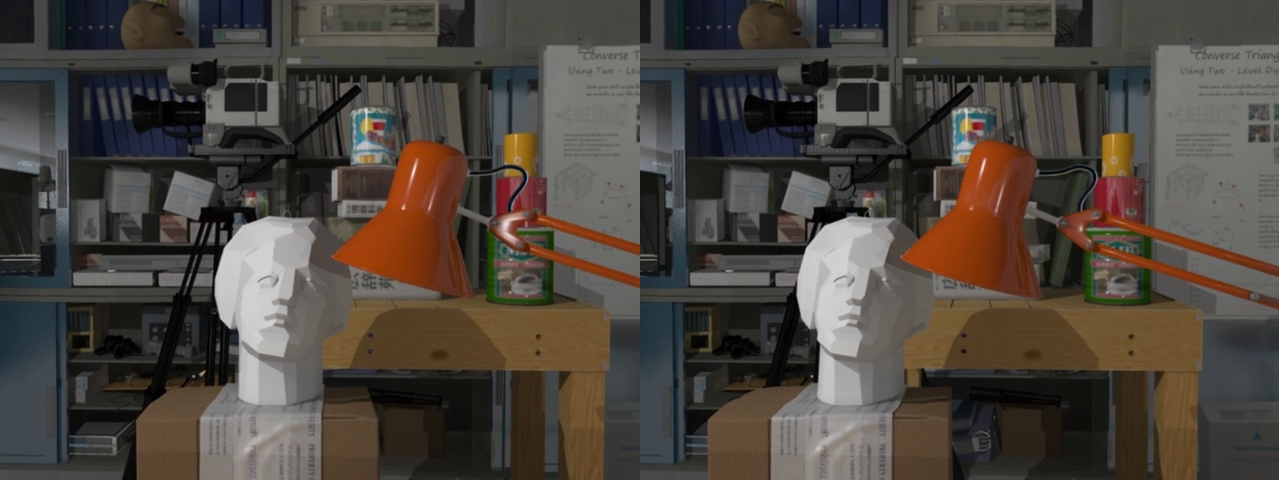
\includegraphics[width=0.9\textwidth]{./img/03_crf1_gt.png}
\caption{\small{stereo image from video marked with power 0.3 and compressed with crf equal to 1 }}
\label{fig:03crf1}
\end{figure}
\begin{figure}[h!]
\centering
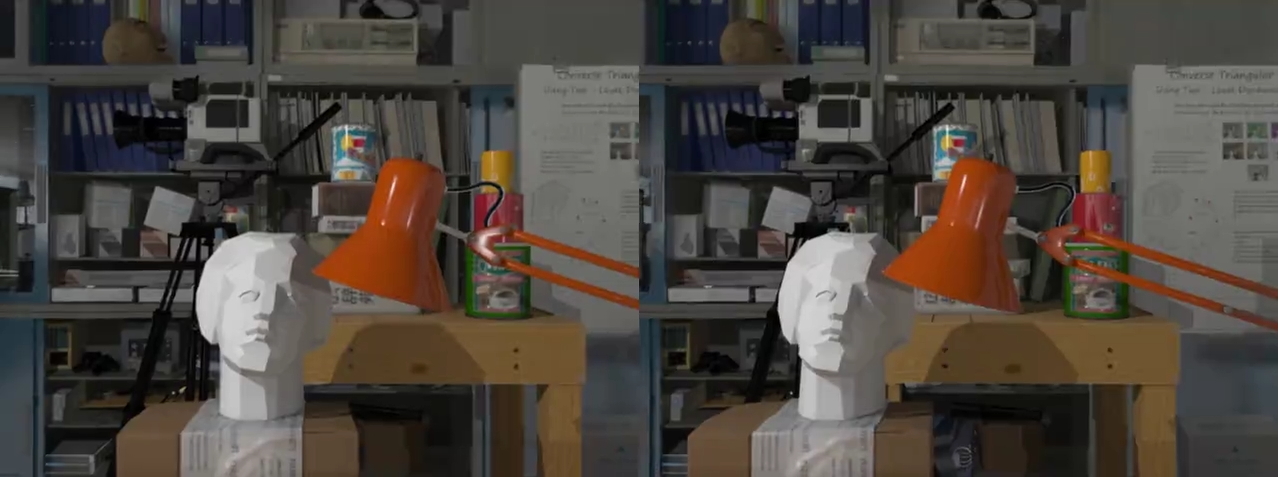
\includegraphics[width=0.9\textwidth]{./img/03_crf30_gt.png}
\caption{\small{stereo image from video marked with power 0.3 and compressed with crf equal to 30 }}
\label{fig:03crf30}
\end{figure}
\begin{figure}[h!]
\centering
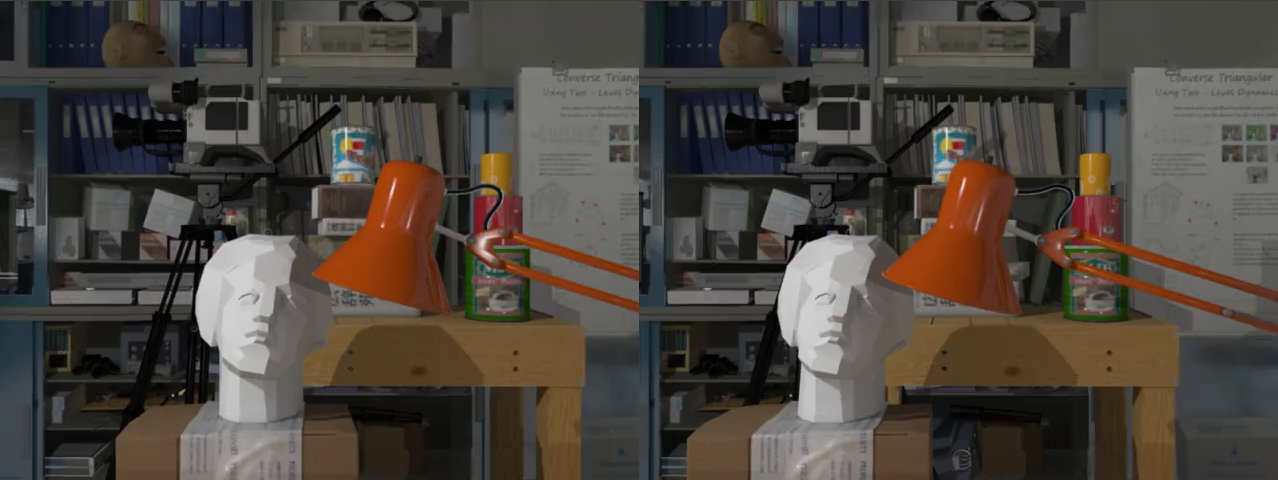
\includegraphics[width=0.9\textwidth]{./img/03_crf25_gt.png}
\caption{\small{stereo image from video marked with power 0.3 and compressed with crf equal to 25 }}
\label{fig:03crf25}
\end{figure}

\begin{figure}[h!]
\centering
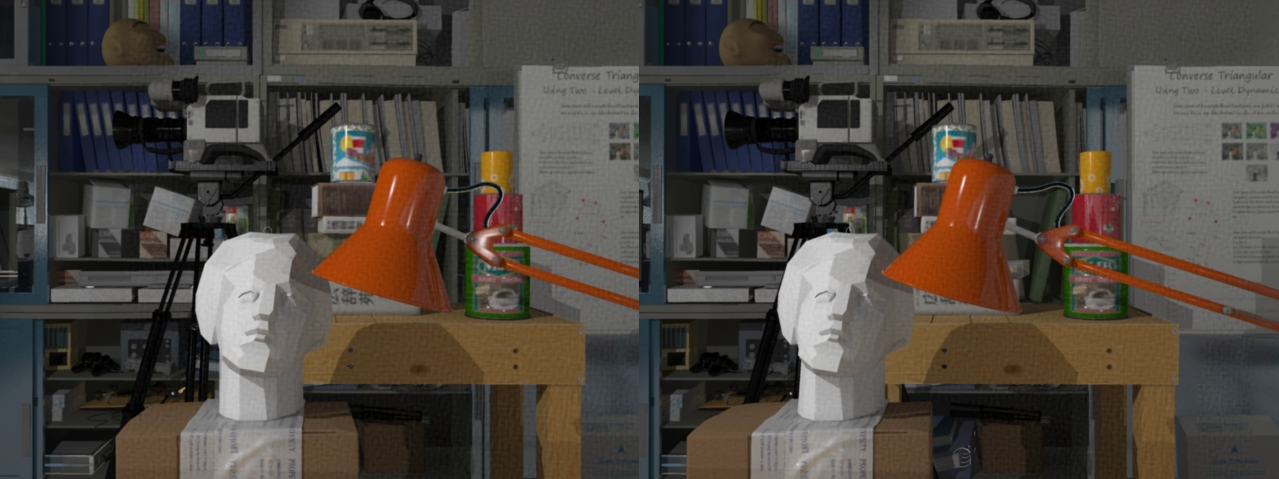
\includegraphics[width=0.9\textwidth]{./img/06_crf1_gt.png}
\caption{\small{stereo image from video marked with power 0.6 and compressed with crf equal to 1 }}
\label{fig:06crf1}
\end{figure}
\begin{figure}[h!]
\centering
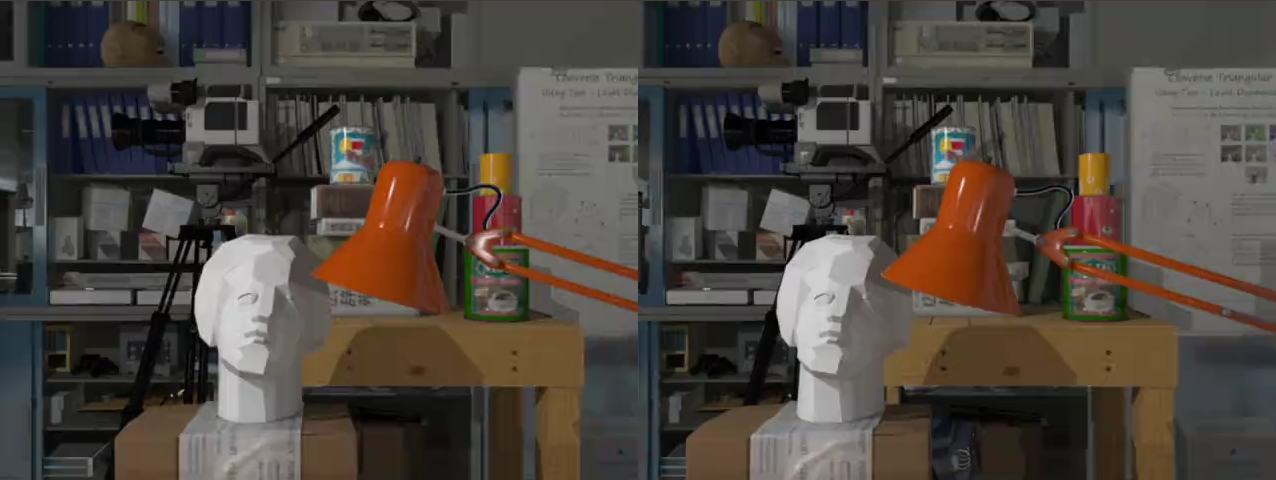
\includegraphics[width=0.9\textwidth]{./img/06_crf30_gt.png}
\caption{\small{stereo image from video marked with power 0.6 and compressed with crf equal to 30 }}
\label{fig:06crf30}
\end{figure}
\begin{figure}[h!]
\centering
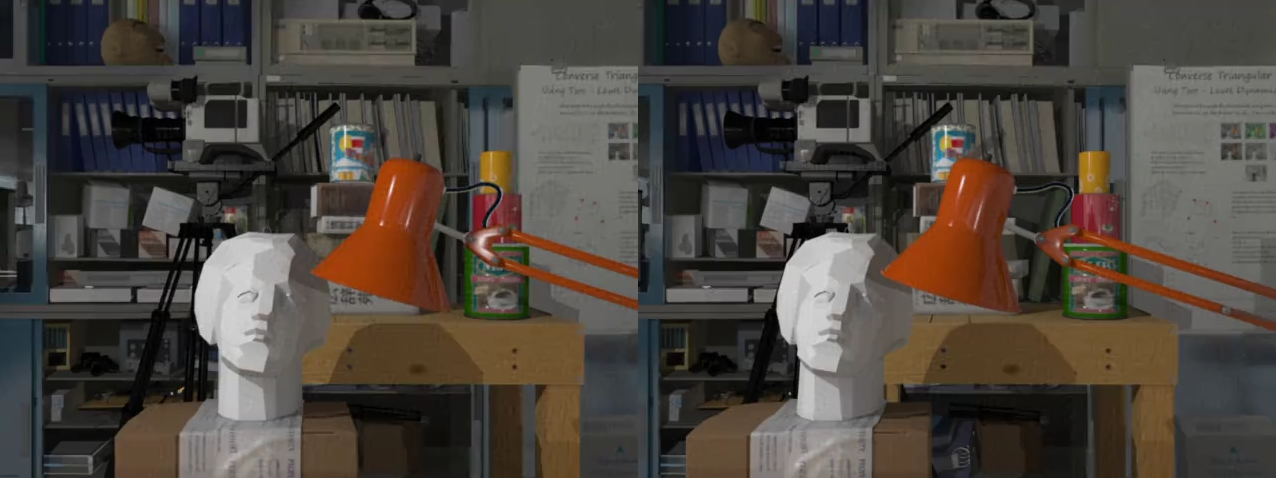
\includegraphics[width=0.9\textwidth]{./img/06_crf25_gt.png}
\caption{\small{stereo image from video marked with power 0.6 and compressed with crf equal to 25 }}
\label{fig:06crf25}
\end{figure}
\clearpage

\subsection{Robusteness in spatial watermarking}

In spatial domain watermarking systems, the watermark is embedded directly in the spatial domain (pixel domain).\newline  Many of the spatial watermarking techniques provide simple and effective schemes for embedding an invisible watermark into an image, but are less robust to common attacks such as lossy compression.

The evaluation of this detection system has been studied through the ROC curve has said in chapter 3. The results are in figures \ref{fig:g1crf}-\ref{fig:g3crf30}.
\begin{figure}[h!]
\centering
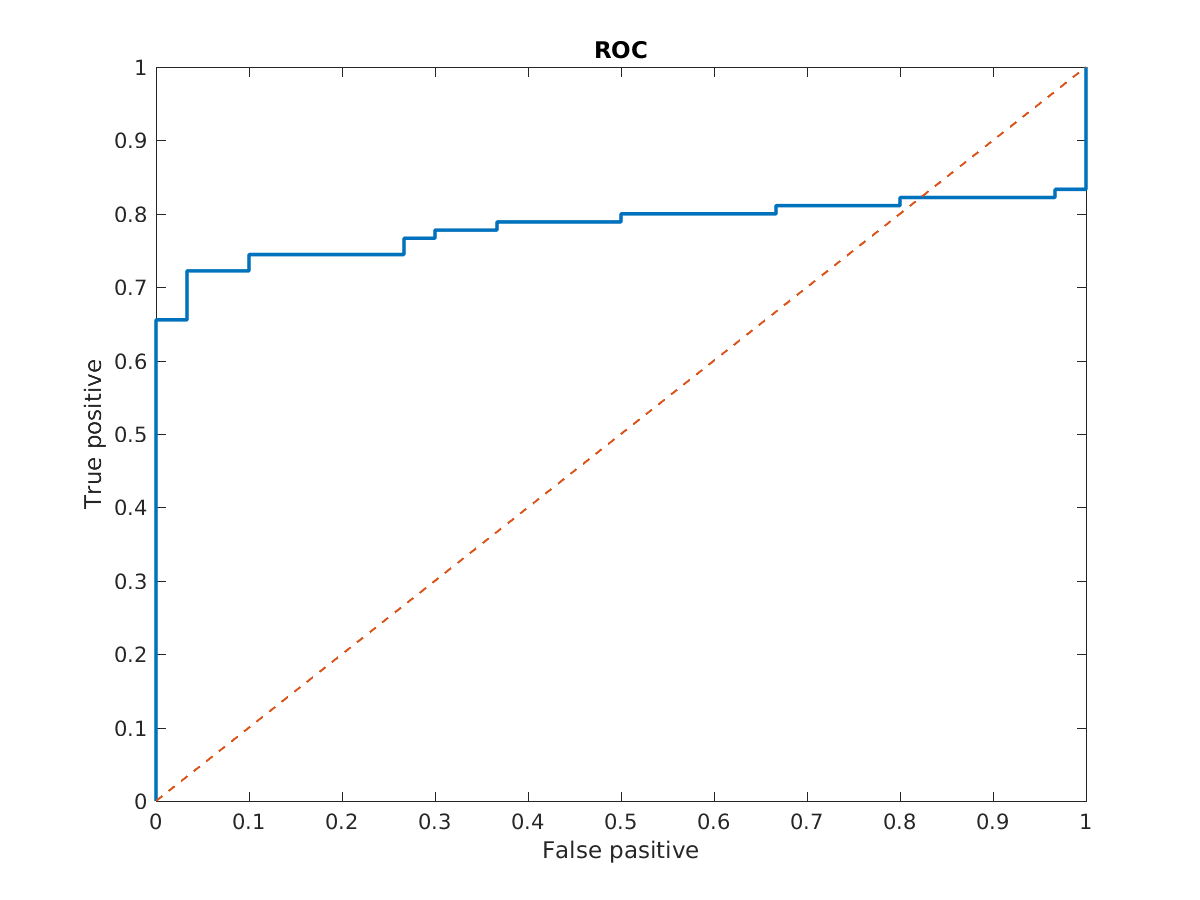
\includegraphics[width=0.4\textwidth]{./img/ROC/ROC_gauss_1_1.png}
\caption{\small{ROC curve of a spatial marked image with power equal to 1 and not compressed}}
\label{fig:g1crf1}
\end{figure}
\begin{figure}[h!]
\centering
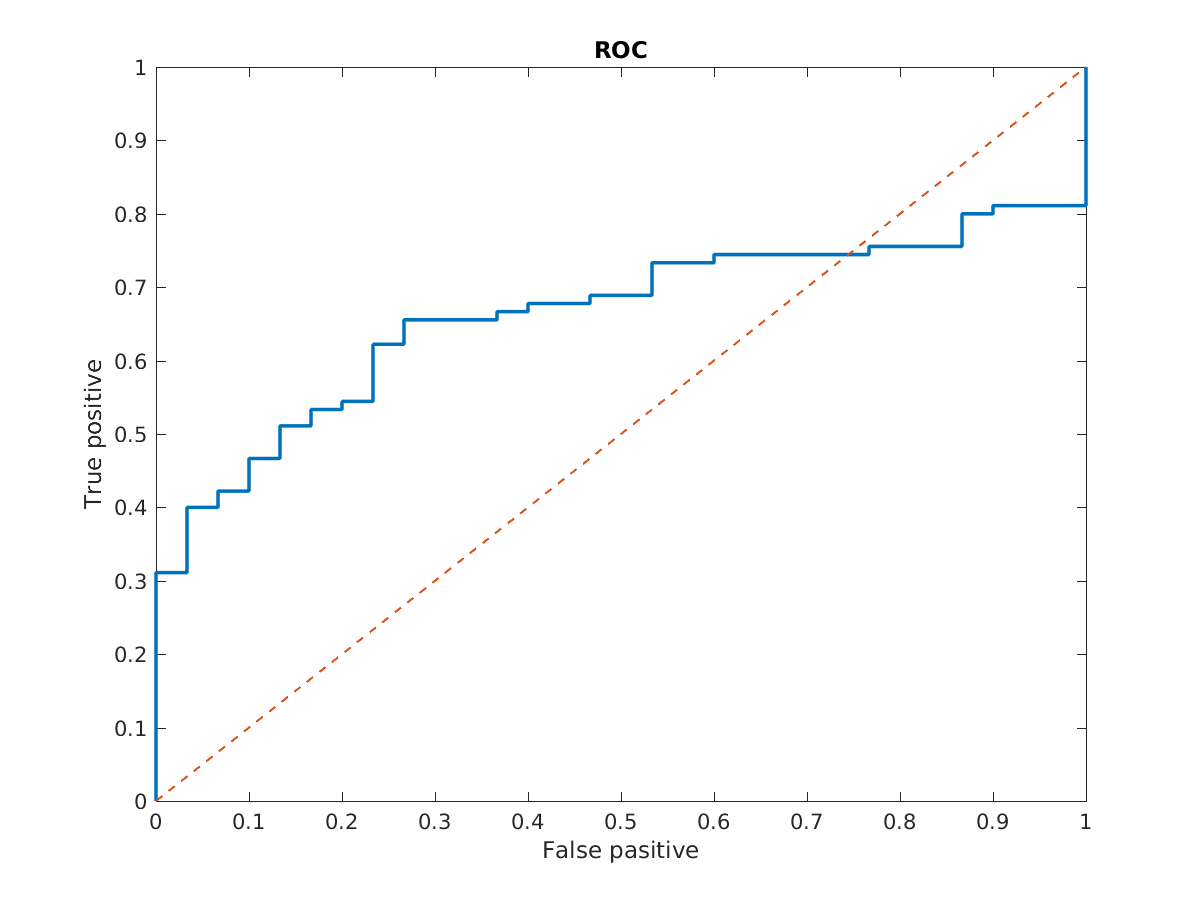
\includegraphics[width=0.4\textwidth]{./img/ROC/ROC_gauss_1_15.png}
\caption{\small{ROC curve of a spatial marked image with power equal to 1 and compressed with crf 15}}
\label{fig:g1crf15}
\end{figure}
\begin{figure}[h!]
\centering
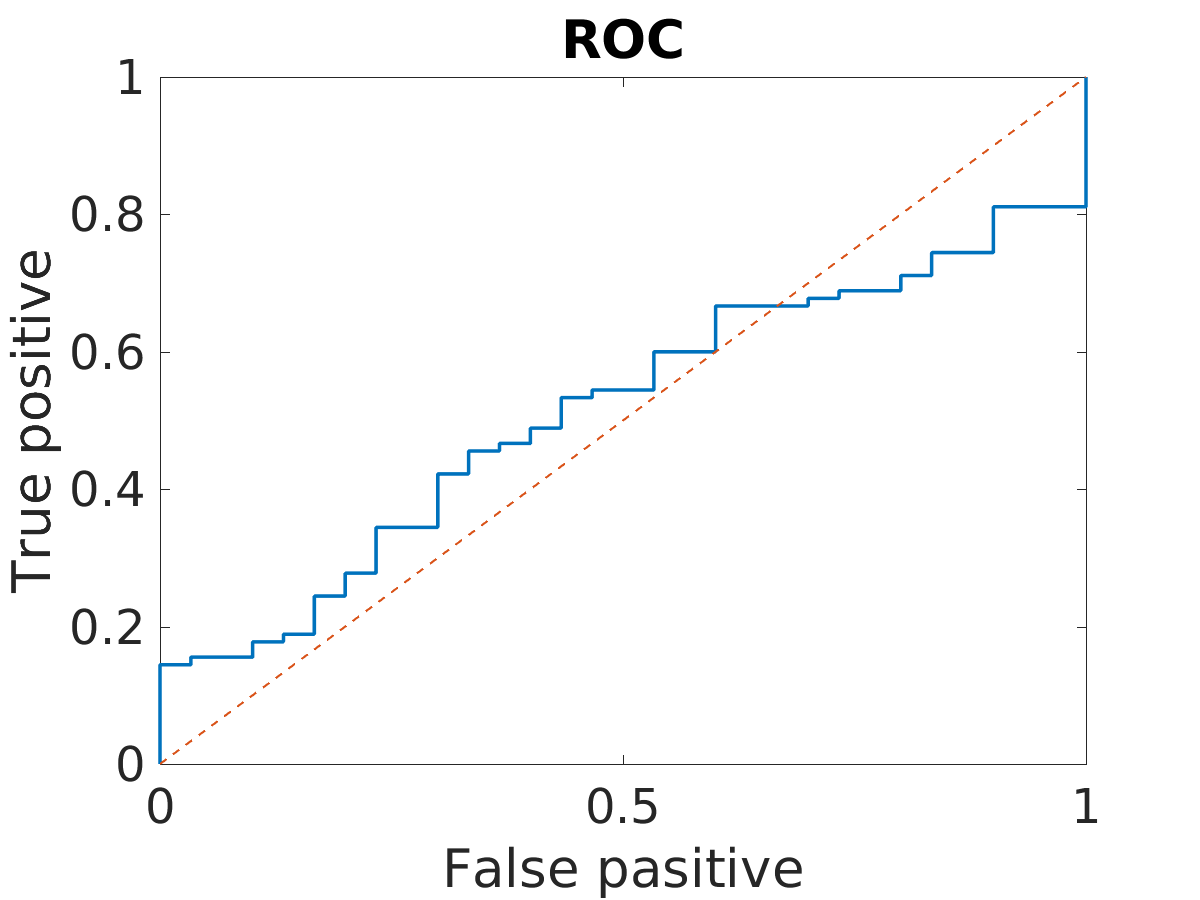
\includegraphics[width=0.4\textwidth]{./img/ROC/ROC_gauss_1_25.png}
\caption{\small{ROC curve of a spatial marked image with power equal to 1 and compressed with crf 25}}
\label{fig:g1crf25}
\end{figure}
\begin{figure}[h!]
\centering
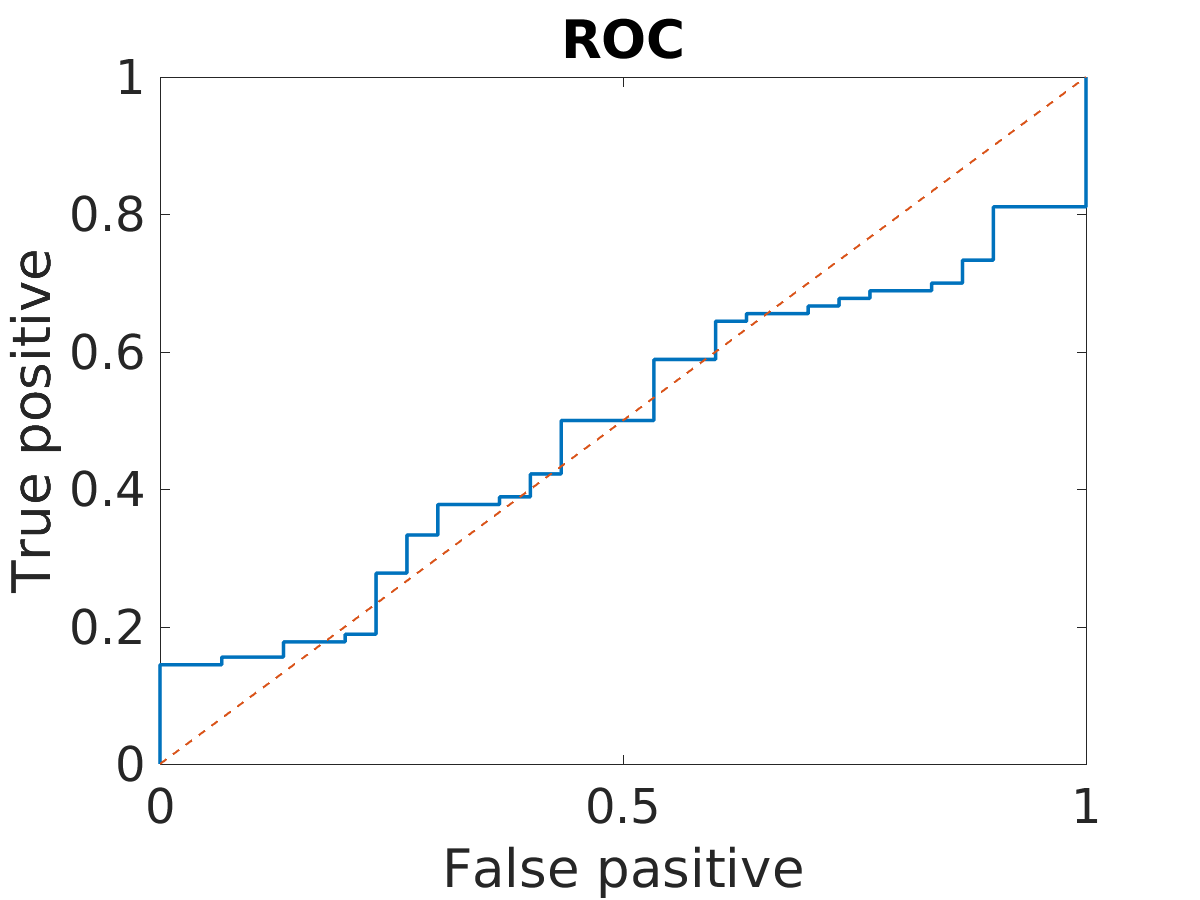
\includegraphics[width=0.4\textwidth]{./img/ROC/ROC_gauss_1_30.png}
\caption{\small{ROC curve of a spatial marked image with power equal to 1 and compressed with crf 30}}
\label{fig:g1crf30}
\end{figure}
\begin{figure}[h!]
\centering
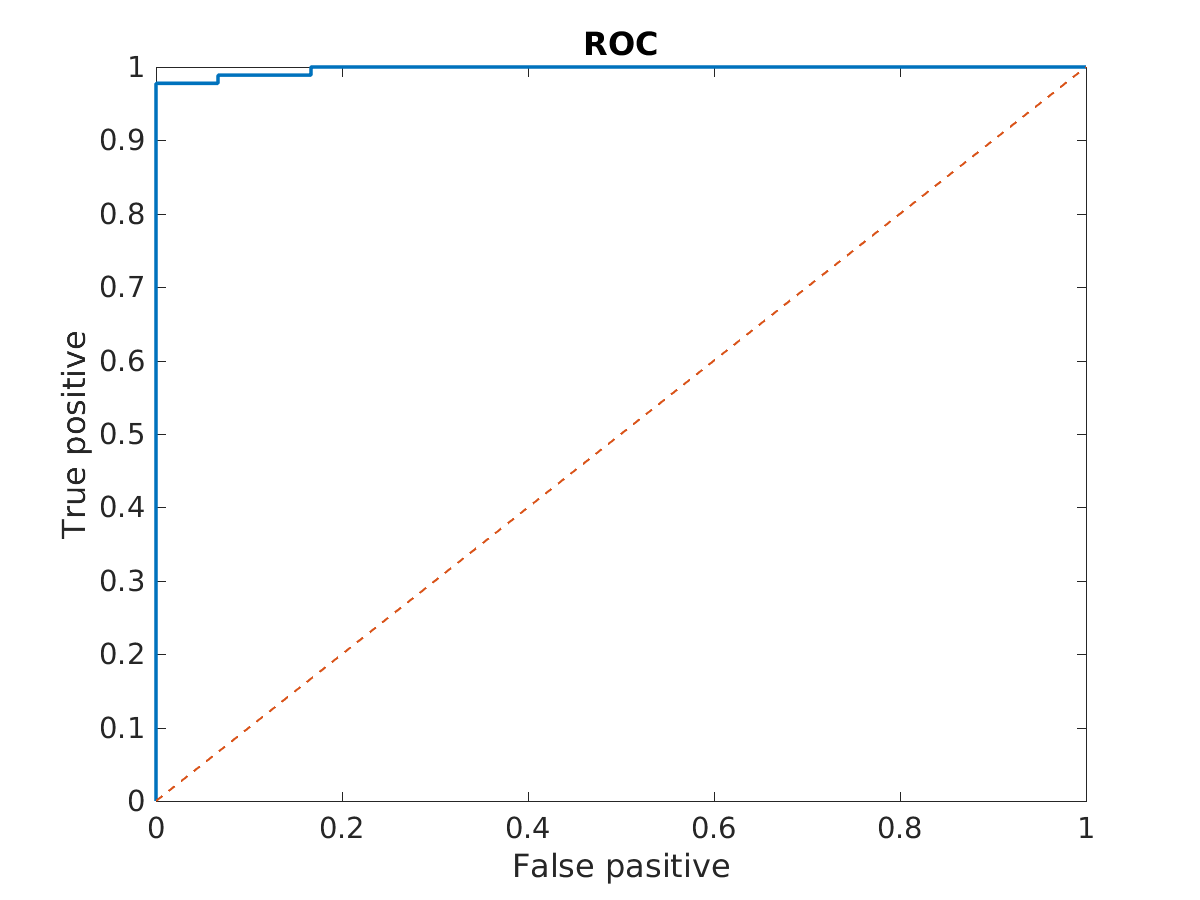
\includegraphics[width=0.4\textwidth]{./img/ROC/ROC_gauss_3_1.png}
\caption{\small{ROC curve of a spatial marked image with power equal to 3 and not compressed }}
\label{fig:g3crf1}
\end{figure}
\begin{figure}[h!]
\centering
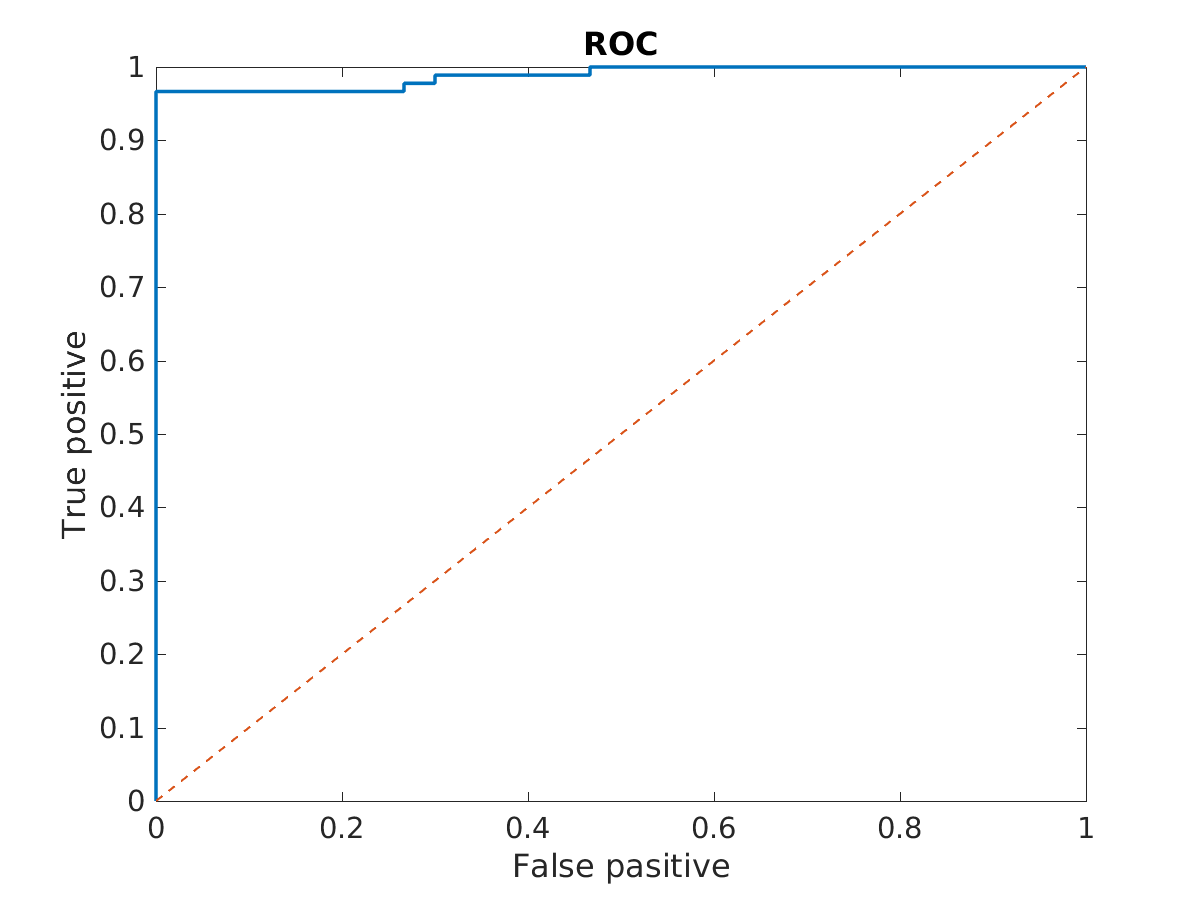
\includegraphics[width=0.4\textwidth]{./img/ROC/ROC_gauss_3_15.png}
\caption{\small{ROC curve of a spatial marked image with power equal to 3 and compressed with crf 15 }}
\label{fig:g3crf15}
\end{figure}
\begin{figure}[h!]
\centering
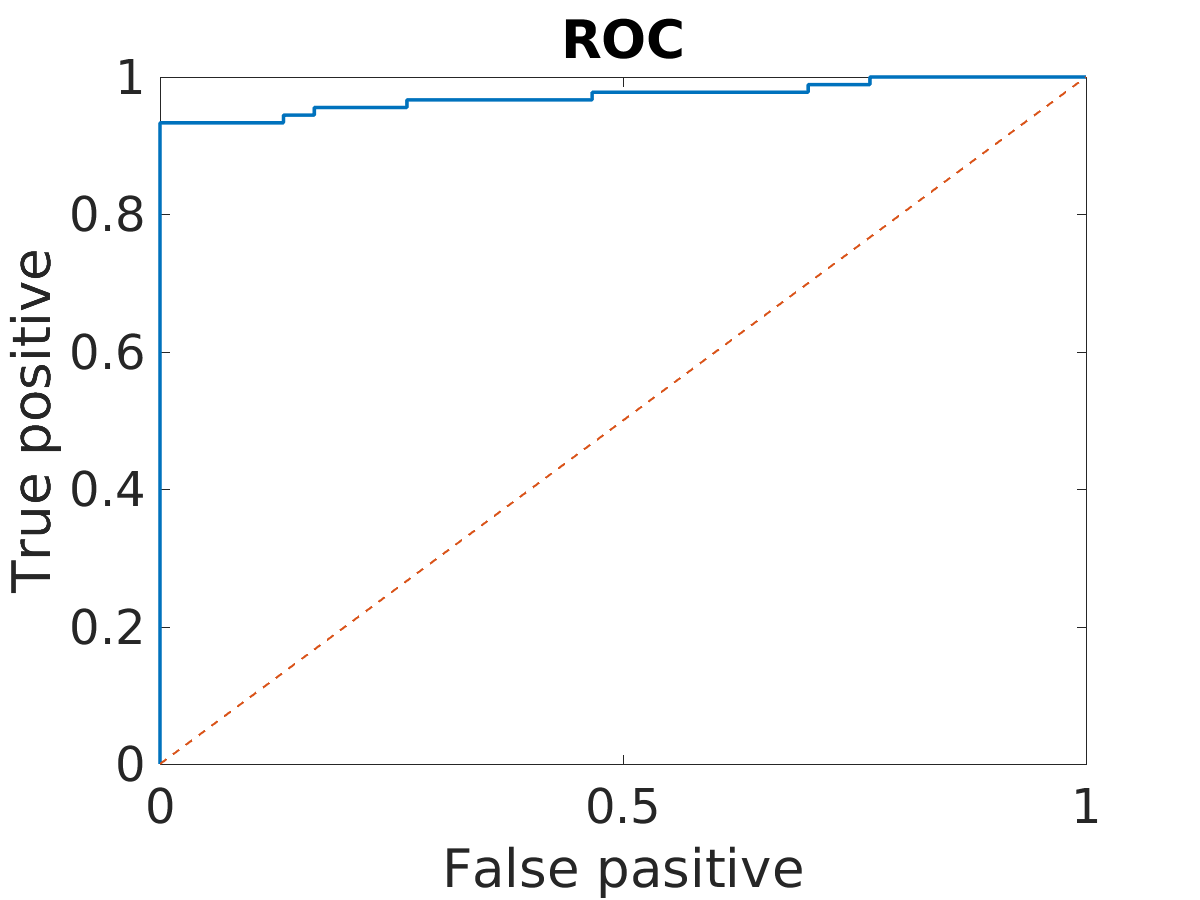
\includegraphics[width=0.4\textwidth]{./img/ROC/ROC_gauss_3_25.png}
\caption{\small{ROC curve of a spatial marked image with power equal to 3 and compressed with crf 25 }}
\label{fig:g3crf25}
\end{figure}
\begin{figure}[h!]
\centering
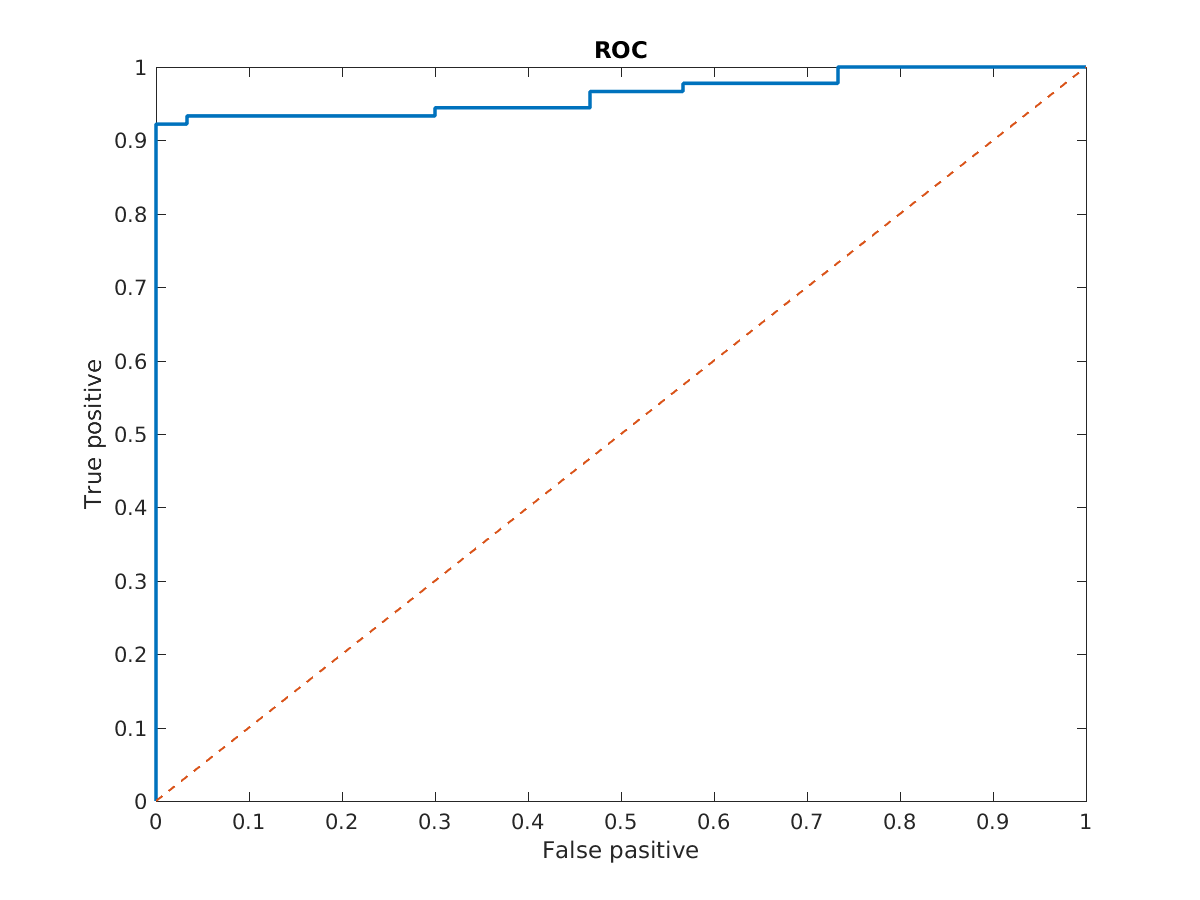
\includegraphics[width=0.4\textwidth]{./img/ROC/ROC_gauss_3_30.png}
\caption{\small{ROC curve of a spatial marked image with power equal to 3 and compressed with crf 30 }}
\label{fig:g3crf30}
\end{figure}
\clearpage
\subsection{Robustess in DFT watermaking}

In transform domain watermarking systems, watermark insertion is done by transforming the image into the frequency domain using a discrete Fourier transform (DFT), full-image DCT, block-wise DCT, wavelet, Hadamard, Fourier-Mellin, or other transforms.\newline  It is often claimed that embedding in the transform domain is advantageous in terms of visibility and security.
 
Two studies are presented in this section: the first one concernes the power of the watermark needed in order to achieve robustness against different levels of compression; the latter focus on youtube, and tries to find the right power to achive robustness in a downloaded video.
 
Each test has been made with both the ground truth and graph-cuts disparities.
 
Tables \ref{tab:compgt}-\ref{tab:compkz} shows how the algorithm manage to find the watermark in a compressed video, in particular it is shown if the mark is detected in the left/right view or both images. The first table shows the results when the algorithm is used with the ground truth disparity, the second when using graph cuts.


\begin{table}[htbp]

 \begin{center}
 \scalebox{0.6}{ 
 \begin{tabular}{c|c|c c c }
 \hline\hline
 \multirow{1}{2.5cm}{\textbf{power}}&\multirow{1}{4cm}{\textbf{compression level}} & \multicolumn{1}{c}{\textbf{both}} & \multicolumn{1}{c}{\textbf{left}} & \multicolumn{1}{c}{\textbf{right}}\\ \hline
 
 0.3 & 1 & 30 & 0 & 0 \\
 0.3 & 15 & 30 & 0 & 0 \\
 0.3 & 25 & 10 & 5 & 0 \\
 0.3 & 30 & 1 & 1 & 0 \\
 0.6 & 1 & 30 & 0 & 0 \\
 0.6 & 15 & 30 & 0 & 0 \\
 0.6 & 25 & 28 & 0 & 0 \\
 0.6 & 30 & 16 & 2 & 0 \\
           
 \hline
 \end{tabular}
 }
 \caption{ \label{tab:compgt}}
 \end{center}
 \end{table}

\begin{table}[htbp]

 \begin{center}
 \scalebox{0.6}{ 
 \begin{tabular}{c|c|c c c }
 \hline\hline
 \multirow{1}{2.5cm}{\textbf{power}}&\multirow{1}{4cm}{\textbf{compression level}} & \multicolumn{1}{c}{\textbf{both}} & \multicolumn{1}{c}{\textbf{left}} & \multicolumn{1}{c}{\textbf{right}}\\ \hline
 
 0.3 & 1 & 30 & 0 & 0 \\
 0.3 & 15 & 29 & 1 & 0 \\
 0.3 & 25 & 11 & 1 & 0 \\
 0.3 & 30 & 2 & 1 & 0 \\
 0.5 & 1 & 30 & 0 & 0 \\
 0.5 & 15 & 30 & 0 & 0 \\
 0.5 & 25 & 24 & 2 & 0 \\
 0.5 & 30 & 9 & 2 & 0 \\
 0.6 & 1 & 30 & 0 & 0 \\
 0.6 & 15 & 30 & 0 & 0 \\
 0.6 & 25 & 26 & 1 & 1 \\
 0.6 & 30 & 15 & 4 & 0 \\
           
 \hline
 \end{tabular}
 }
 \caption{ \label{tab:compkz}}
 \end{center}
 \end{table}
 
Figures \ref{fig:03yt}-\ref{fig:08yt} show how the uploading and the subsequential download of a non compressed video on youtube degradates the image.\newline
 
\begin{figure}[h!]
\centering
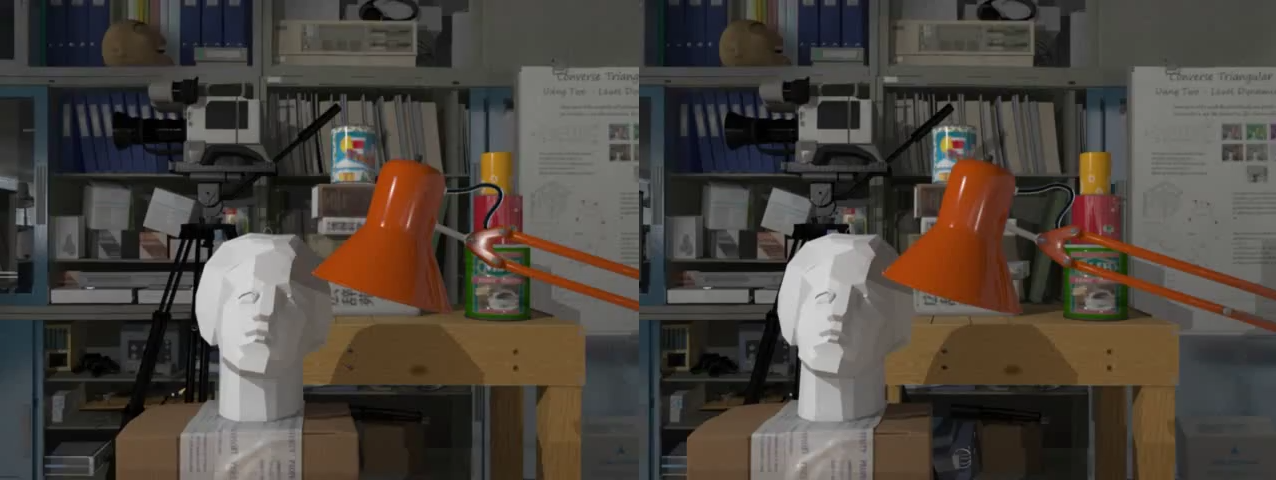
\includegraphics[width=0.9\textwidth]{./img/yt_03_gt.png}
\caption{\small{stereo image from video uploaded with power equal to 0.3 }}
\label{fig:03yt}
\end{figure}
\begin{figure}[h!]
\centering
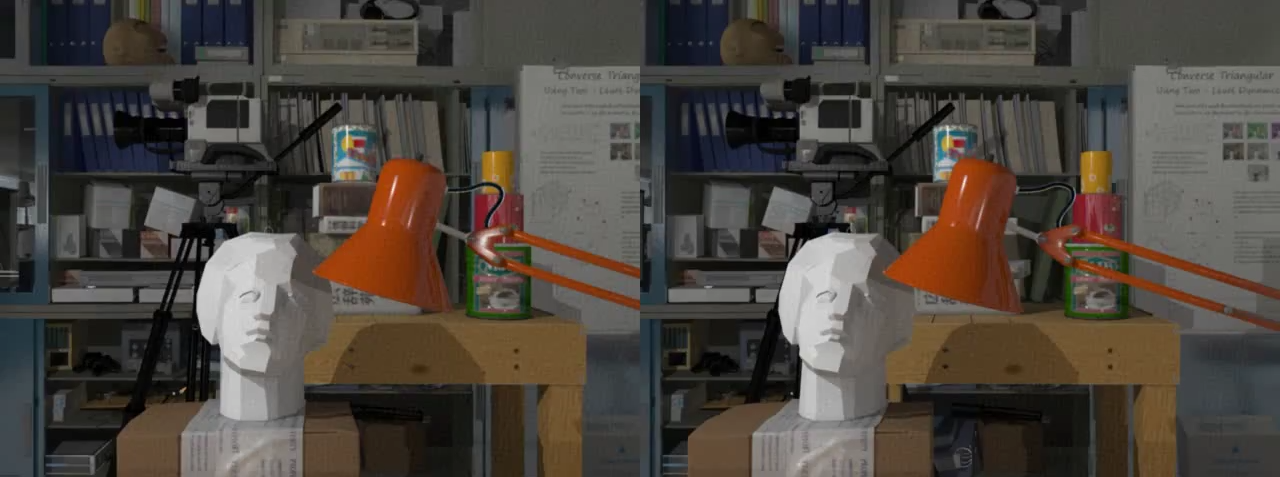
\includegraphics[width=0.9\textwidth]{./img/yt_06_gt.png}
\caption{\small{stereo image from video uploaded with power equal to 0.6 }}
\label{fig:06yt}
\end{figure}
\begin{figure}[h!]
\centering
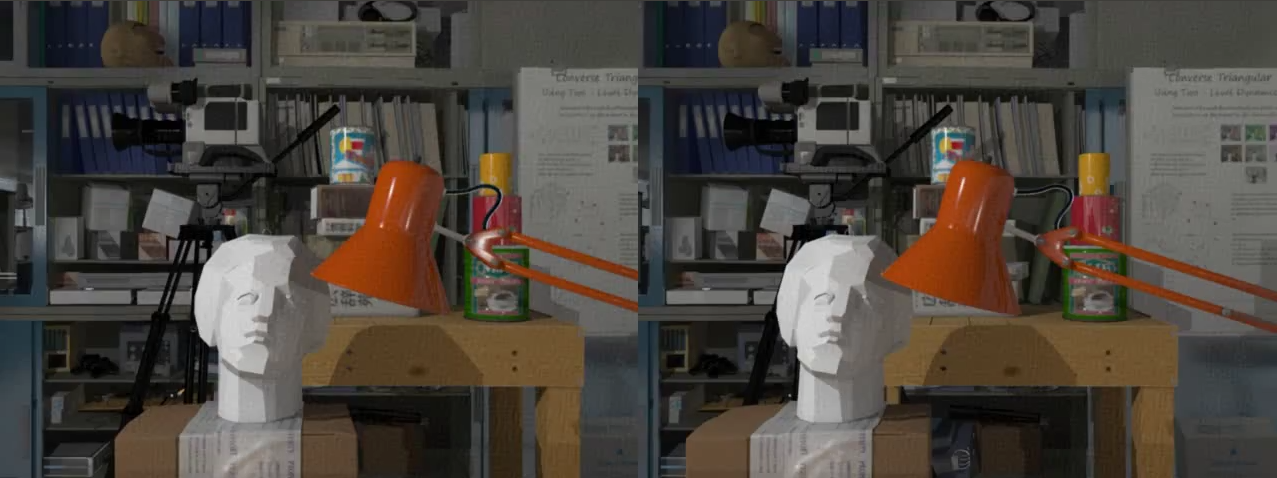
\includegraphics[width=0.9\textwidth]{./img/yt_07_gt.png}
\caption{\small{stereo image from video uploaded with power equal to 0.7 }}
\label{fig:07yt}
\end{figure}
\begin{figure}[h!]
\centering
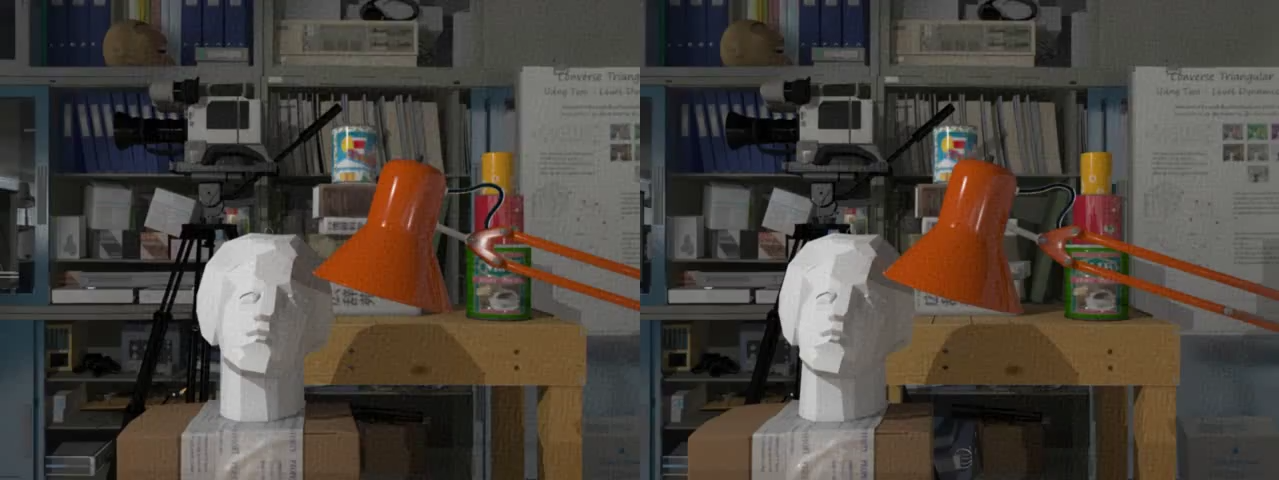
\includegraphics[width=0.9\textwidth]{./img/yt_08_gt.png}
\caption{\small{stereo image from video uploaded with power equal to 0.8 }}
\label{fig:08yt}
\end{figure}
\clearpage

Tables \ref{tab:ytgt}-\ref{tab:ytkz} show how a video uploaded on youtube and subsequentially downloaded can preserve the watermark, respectively when the watermark is inserted with the ground truth disparity and with graph cuts.\newline
 
 
 \begin{table}[htbp]

  \begin{center}
  \scalebox{0.6}{ 
  \begin{tabular}{c|c c c }
  \hline\hline
  \multirow{1}{2.5cm}{\textbf{power}} & \multicolumn{1}{c}{\textbf{both}} & \multicolumn{1}{c}{\textbf{left}} & \multicolumn{1}{c}{\textbf{right}}\\ \hline
 0.3 & 1 & 0 & 0\\
 0.6 & 9 & 1 & 0\\
 0.7 & 12& 2 & 0\\
 0.8 & 16& 0 & 1\\ 
  \hline
  \end{tabular}
  }
  \caption{\label{tab:ytgt}}
  \end{center}
  \end{table}
 
\begin{table}[htbp]
 
 \begin{center}
 \scalebox{0.6}{ 
 \begin{tabular}{c|c c c }
 \hline\hline
 \multirow{1}{2.5cm}{\textbf{power}} & \multicolumn{1}{c}{\textbf{both}} & \multicolumn{1}{c}{\textbf{left}} & \multicolumn{1}{c}{\textbf{right}}\\ \hline

0.3& 1& 0& 0\\
0.5& 6 & 1& 0\\
0.6& 11 & 0 & 0\\
 \hline
 \end{tabular}
 }
 \caption{\label{tab:ytkz}}
 \end{center}
 \end{table}


One can notice that, at a global level, detection  statistics gradually degrade with the compression ratio. The embedded watermark becomes hardly detectable at the crudest compression levels even with if embedded with a strong power. 
 \clearpage
 
\section{Robustness to View Synthesis}

In a second batch of experiments, we analyzed the impact of virtual view synthesis on the detection performances of our watermarking system. To this end, we generated a number of intermediate synthetic views (figures \ref{fig:synt1/4}-\ref{fig:synt3/4}), equally spaced apart between the left (reference) view and the right one, using the code in [].\newline

\begin{figure}[h!]
\centering
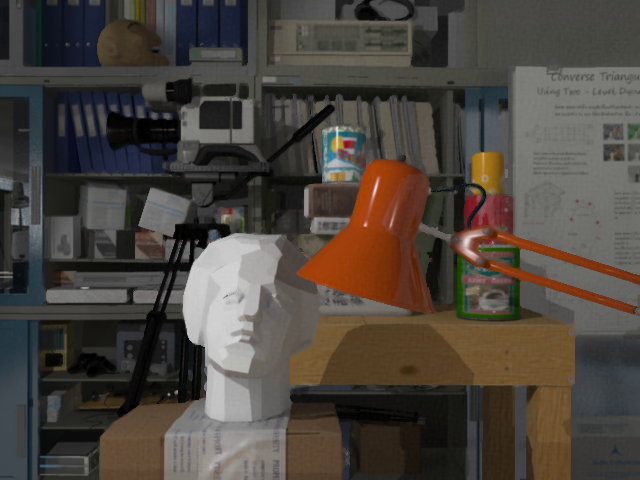
\includegraphics[width=0.5\textwidth]{./img/synth_view1_25.png}
\caption{\small{synthetized view at distance 1/4 of the baseline from the left image }}
\label{fig:synt1/4}
\end{figure}
\begin{figure}[h!]
\centering
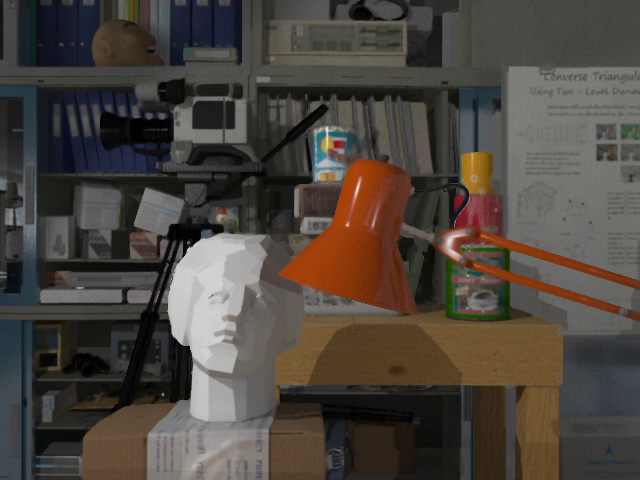
\includegraphics[width=0.5\textwidth]{./img/synth_view1_50.png}
\caption{\small{synthetized view at distance 1/2 of the baseline from the left image }}
\label{fig:synt1/2}
\end{figure}
\begin{figure}[h!]
\centering
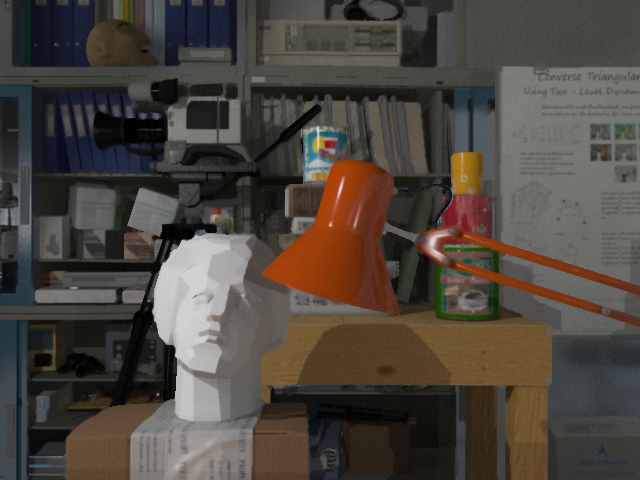
\includegraphics[width=0.5\textwidth]{./img/synth_view1_75.png}
\caption{\small{synthetized view at distance 3/4 of the baseline from the left image }}
\label{fig:synt3/4}
\end{figure}

The views have been synthetized for both the spatial and frequency method, the result are shown below.\newline
The table \ref{tab:syntDFT} contains the results for the frequency marking: the first column is the distance between the left view and the synthetized one, in terms of fraction of the baseline, then its show in how many synthetized images the mark is detected.

\begin{table}[htbp]

 \begin{center}
 \scalebox{0.6}{ 
 \begin{tabular}{c|c c c }
 \hline\hline
 \multirow{1}{2.5cm}{\textbf{position}} & \multicolumn{1}{c}{\textbf{both}} & \multicolumn{1}{c}{\textbf{left}} & \multicolumn{1}{c}{\textbf{right}}\\ \hline

1/2 & 30& 0& 0\\
1/4 & 30& 0& 0\\
3/4 & 29 & 1 & 0\\
 \hline
 \end{tabular}
 }
 \caption{ \label{tab:syntDFT}}
 \end{center}
 \end{table}
 
  
The same study is proposed for the spatial marking: from a video marked with additive gaussian noise have been generated three synthetized views for each pair of marked frames, respectively one in the middle and the other two at 1/4 and 3/4 of distance from the left.\newline The ROC curves in figures \ref{fig:g1vs25}-\ref{fig:g3vs75}  show the results for the different intermediate synthetic views.\newline 
\begin{figure}[h!]
\centering
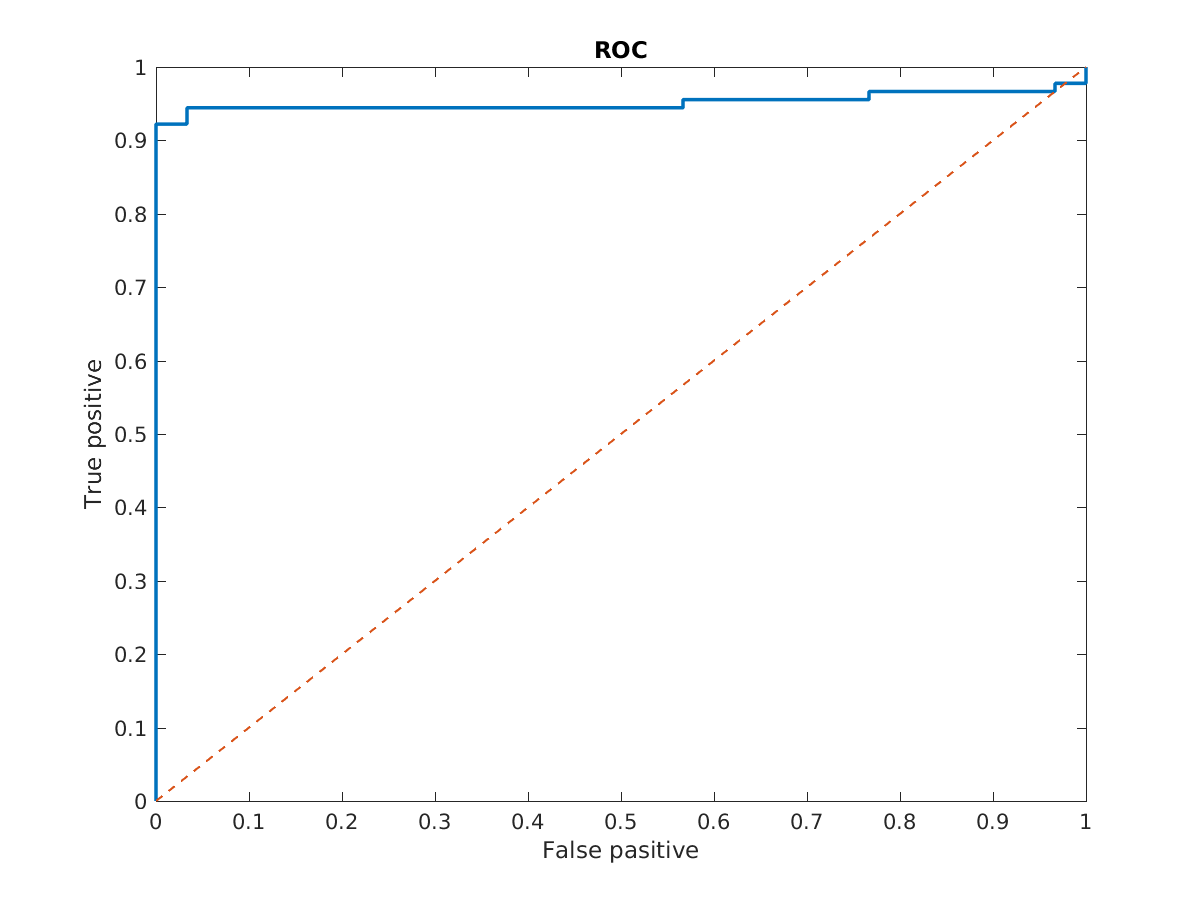
\includegraphics[width=0.4\textwidth]{./img/ROC/ROC_gauss_synt_1_25.png}
\caption{\small{ROC curve of a synthetic view created at distance equal to baseline/4 marked with power equal to 1 }}
\label{fig:g1vs25}
\end{figure}
\begin{figure}[h!]
\centering
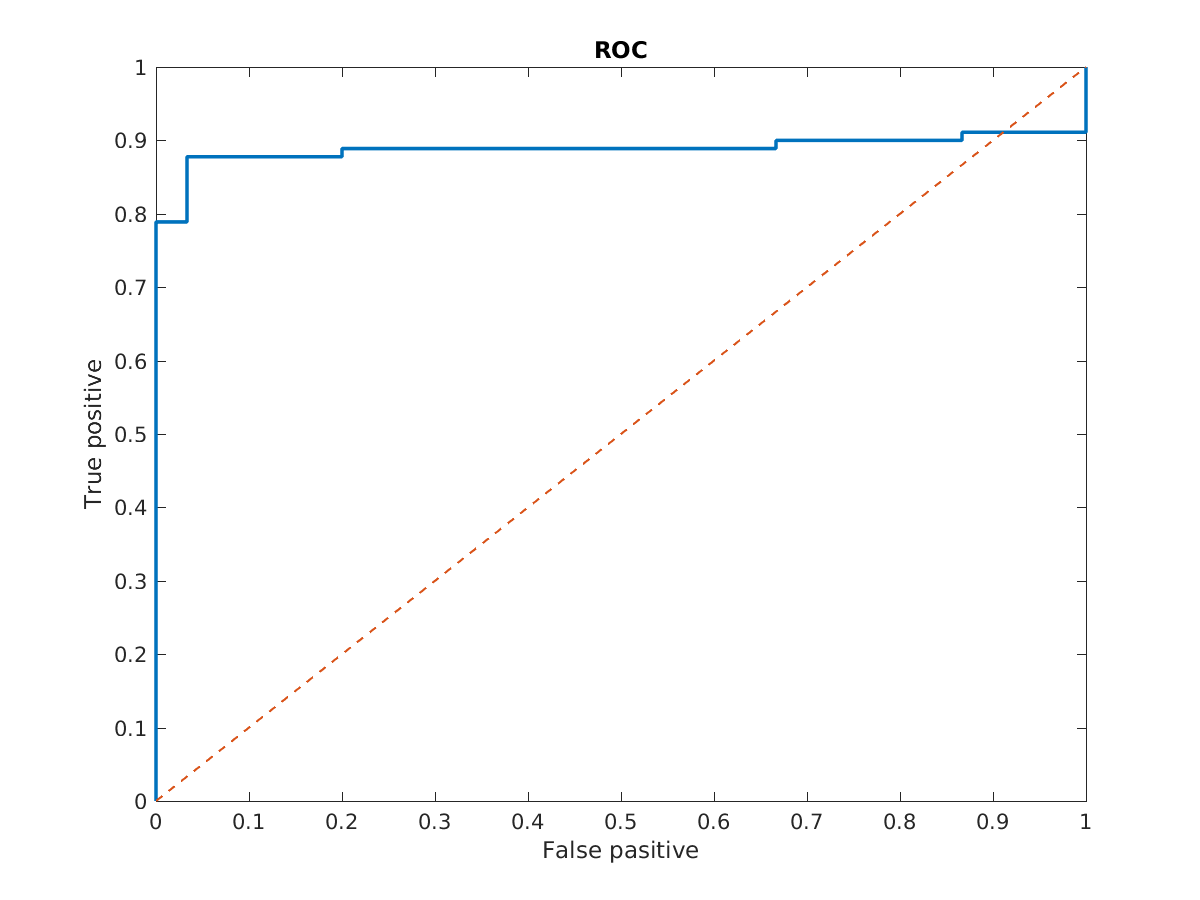
\includegraphics[width=0.4\textwidth]{./img/ROC/ROC_gauss_synt_1_50.png}
\caption{\small{ROC curve of a synthetic view created at distance equal to baseline/2 marked with power equal to 1 }}
\label{fig:g1vs50}
\end{figure}
\begin{figure}[h!]
\centering
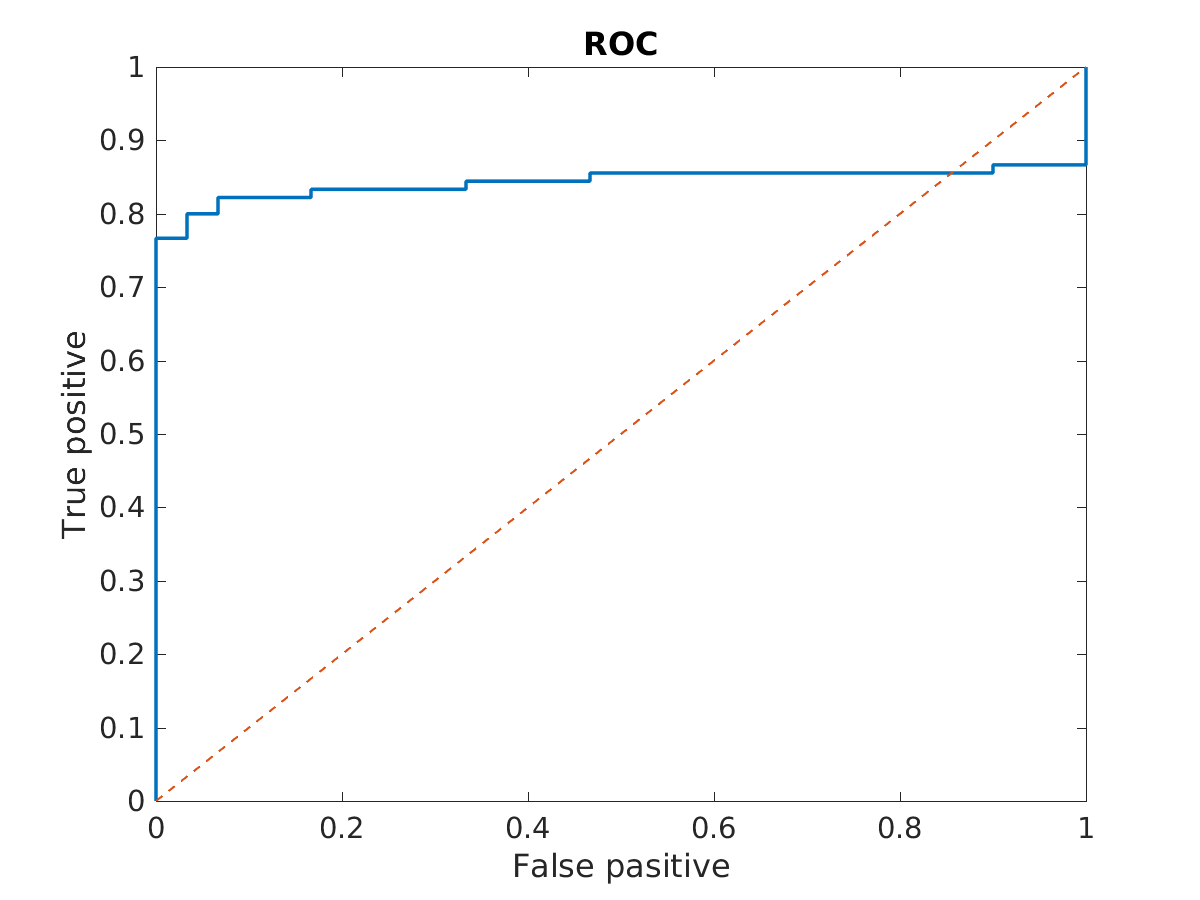
\includegraphics[width=0.4\textwidth]{./img/ROC/ROC_gauss_synt_1_75.png}
\caption{\small{ROC curve of a synthetic view created at distance equal to baseline*3/4 marked with power equal to 1 }}
\label{fig:g1vs75}
\end{figure}
\begin{figure}[h!]
\centering
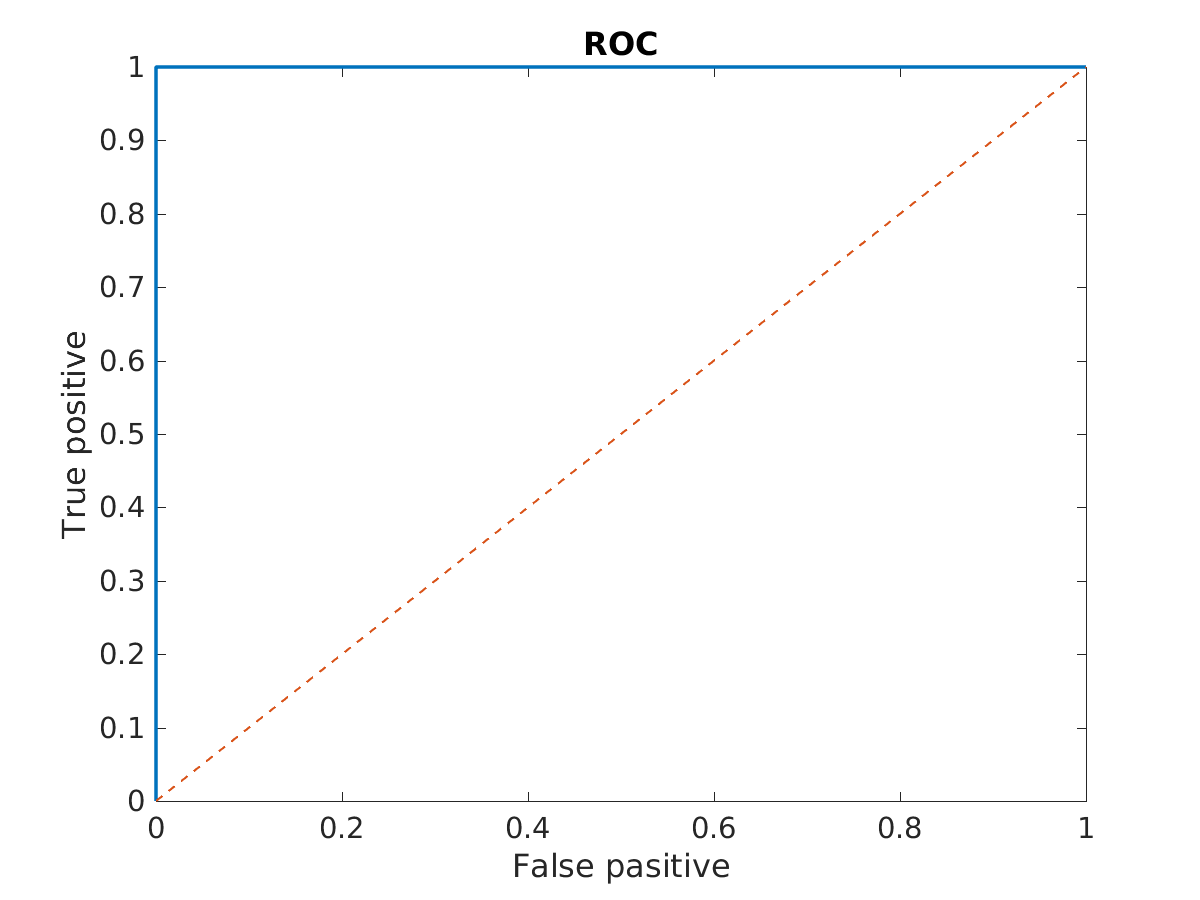
\includegraphics[width=0.4\textwidth]{./img/ROC/ROC_gauss_synt_3_25.png}
\caption{\small{ROC curve of a synthetic view created at distance equal to baseline/4 marked with power equal to 3 }}
\label{fig:g3vs25}
\end{figure}
\begin{figure}[h!]
\centering
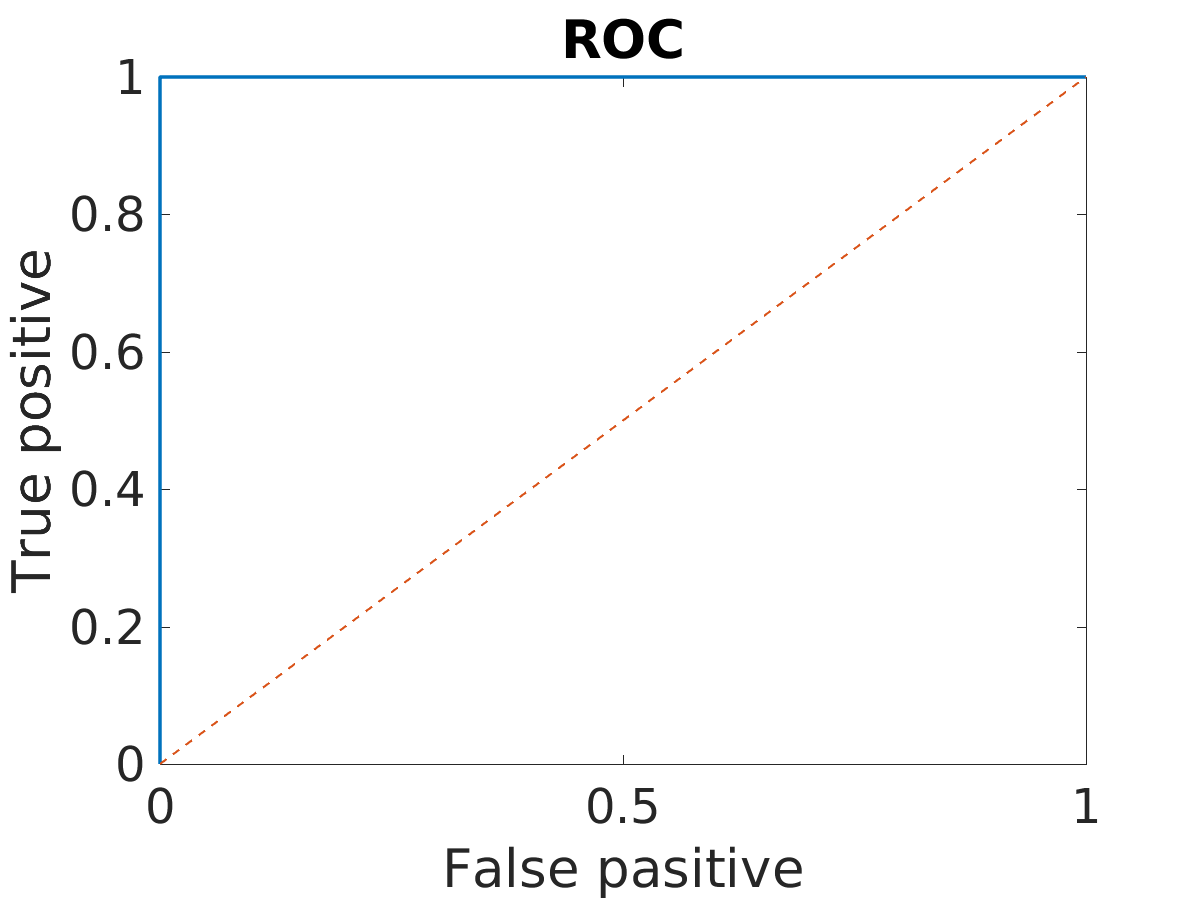
\includegraphics[width=0.4\textwidth]{./img/ROC/ROC_gauss_synt_3_50.png}
\caption{\small{ROC curve of a synthetic view created at distance equal to baseline/2 marked with power equal to 3 }}
\label{fig:g3vs50}
\end{figure}
\begin{figure}[h!]
\centering
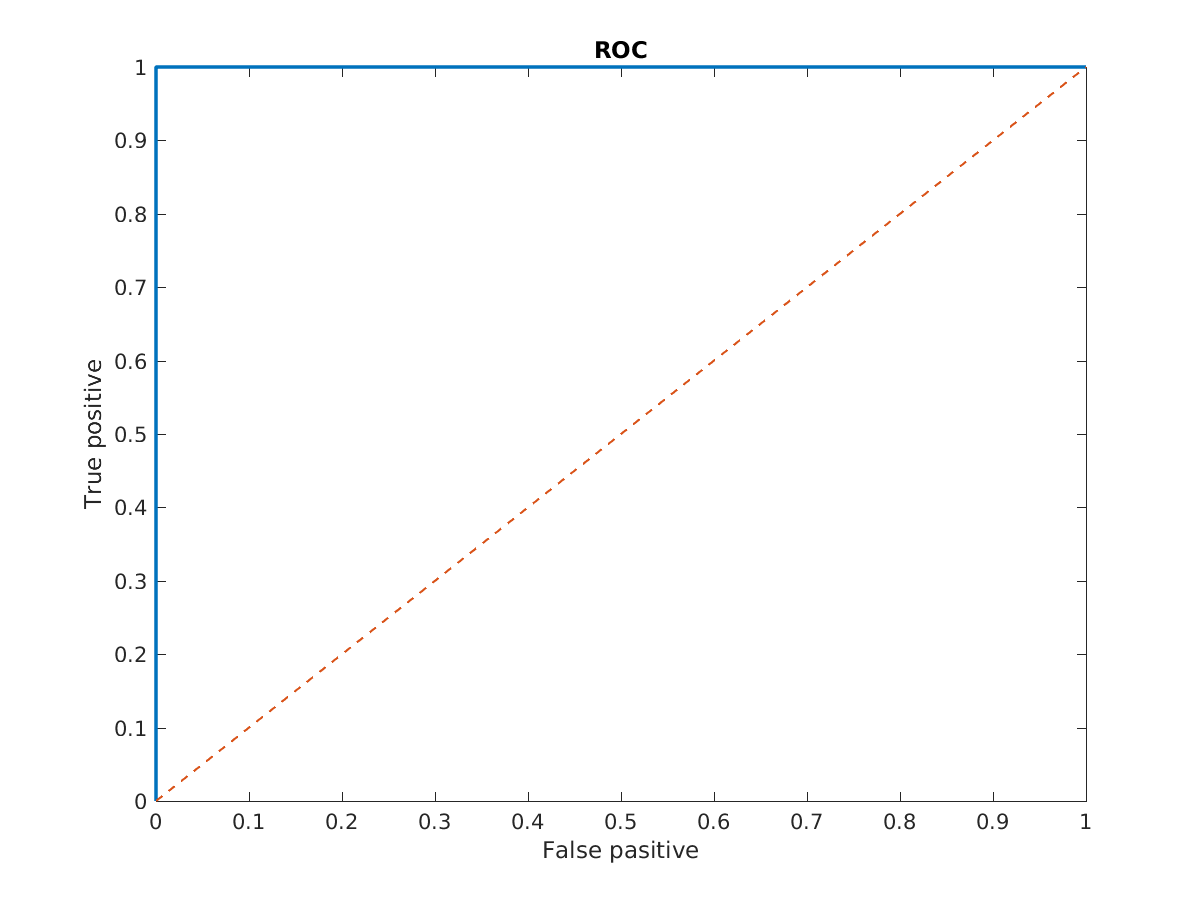
\includegraphics[width=0.4\textwidth]{./img/ROC/ROC_gauss_synt_3_75.png}
\caption{\small{ROC curve of a synthetic view created at distance equal to baseline*3/4 marked with power equal to 3 }}
\label{fig:g3vs75}
\end{figure}
\clearpage
It can be noted that the watermark is always detected in the synthetized views, we can therefore expect the synthetized views to behave like the other against compression.\newline

Often with stereo watermarking, view synthesis can be a problem since local geometric deformations destroys the synchronization necessary for the detection process to be succesful. With the proposed method although the resynchronization is an internal step of the detection process and it doesn't need side information since it is based on the estimation of the disparity map.

\section{Perceptual impact}

As said in chapter 2 the perceptual impact, i.e. the imperceptivity of the watermark to the human eye, has been measure with the metrics proposed by Chaminda et al. These metrics have been used to evaluate the impact of the watermark with a RR method, instead of the compression degradation as in \cite{METRICS}.

For different power of watermarking both the $MQ_{depth}$ and $MQ_{color}$ metrics are calculated, and in figures \ref{fig:} its shown the value of the quality measure with respect to the power of the embedded watermark.   


